\documentclass[12pt]{article}\usepackage[left=20mm,right=20mm,top=15mm,bottom=20mm]{geometry}

\usepackage[T1]{fontenc}
\usepackage[magyar]{babel}
\usepackage[utf8]{inputenc}
\usepackage[table,xcdraw]{xcolor}

\usepackage{graphicx}
\usepackage{caption}
\usepackage{siunitx}
\usepackage{amsmath}
\usepackage{pdflscape}
\usepackage{epstopdf}
\usepackage{multirow}
\usepackage{makeidx}
\usepackage{placeins}
\usepackage{subcaption}
\usepackage{hyperref}

%\DeclareUnicodeCharacter{00A0}{~}

\begin{document}
\begin{titlepage}
\centering
	
\includegraphics[width=0.5\textwidth]{figures/bme_logo_kicsi.eps}\par\vspace{1cm}
	\vspace{1cm}
	\vspace{1.5cm}
	{\huge\bfseries Szoftvertervezés 2. házi feladat \par}
	\vspace{15cm}
	{\huge\itshape Locskai Norbert, Kovács András, Barancsuk Lilla \par}
	\vfill

% Bottom of the page
	{\large \today\par}
\end{titlepage}

\thispagestyle{empty}
\begin{landscape}
\section{Domain modell}
%\newgeometry{left=50mm,right=2mm,top=98.5mm,bottom=10mm}
\begin{figure}[!h]
    \centering
        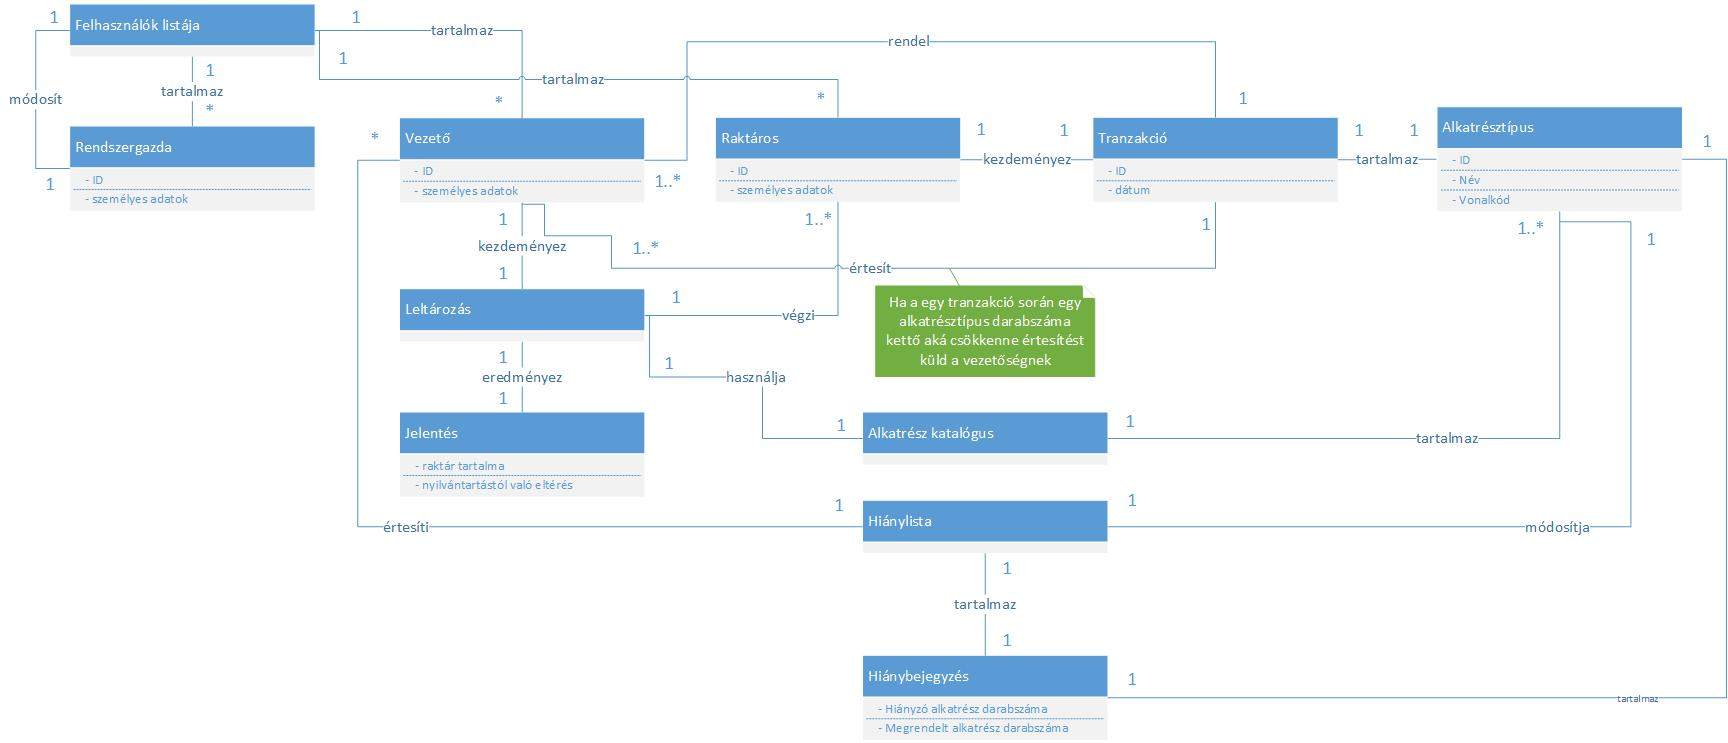
\includegraphics[width=1.4\textwidth]{kepek/Domain_model.jpg}
        \caption{Domain modell.}
\end{figure}
\end{landscape}

\section{Design modell}
\subsection{Use case-ek megvalósítása}
A use case-ek megvalósítását szekvenciadiagramokon ábrázoltuk.

\subsubsection{Rendelés összeállítása}
A rendelést a vezető kezdeményezi, amihez be kell lépnie a  szoftver weber felületén keresztül.
A rendelés alapja a hiányzó alkatrészek listája, amit a céges szerveren tárolt adatbázis szolgáltat. 
A webes felület biztosítja a vezető számára, hogy a hiányzó alkatrészek listájának felhasználásával összeállítsa a rendelést, majd azt többféle formátumban exportálja a felületen keresztül.

\begin{figure}[!h]
    \centering
        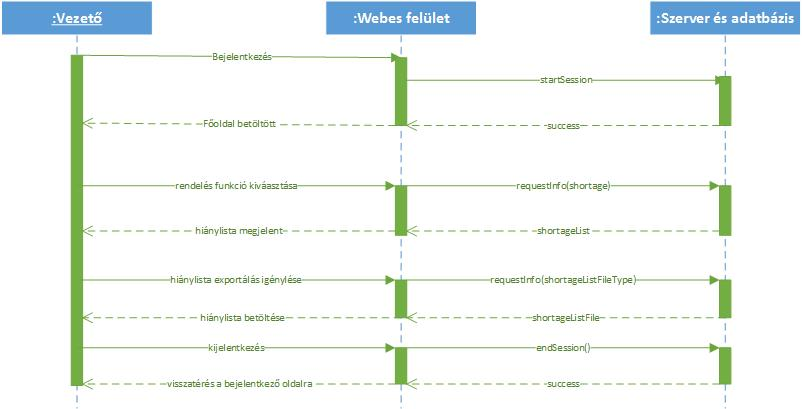
\includegraphics[width=1.4\textwidth]{kepek/Rendeles_szekvencia.jpg}
        \caption{A rendelés szekvencia diagramja.}
\end{figure}

\subsubsection{Alkatrészek kiadása}
Az alkatrészek kiadását a raktáros végzi a szerelő által átadott munkalap alapján. A raktáros az átadott munkalapon szereplő alkatrészeket kiveszi a raktárból, majd a vonalkód-leolvasóval leolvassa ezeket. 
A rendszer összeállít egy listát a kivitt alkatrészekből, és ezeket törli az adatbázisból.
Az esetleges alkatrészhiány kialakulását (amennyiben egy adott típusú alkatrész száma kettő alá csökken) jelzi a vezetőségnek. 

\subsubsection{Leltározás kezdeményezése}

\subsection{Design Class Diagram}



\end{document}